\section{Теоретическая часть}

В радиотехнических приборах требуется осуществить преобразование исходного эксцентрического сигнала, носящее характер дифференцирования или интегрирования. Иными словами, если на взод некоего четырехполюсника должен сниматься сигнал
\begin{align} \label{eq:th:1}
	u_\text{вых} (t) = \tau_0 \frac{du_\text{вх}(t)}{dt}
\end{align}  
а с выхода интегрирующего четырехполюсника -- сигнал
\begin{equation} \label{eq:th:2}
	u_\text{вых}(t) = \frac{1}{\tau_0}\int\limits_{-\infty}^{t} u_\text{вх}(t)\,dt,
\end{equation}
где $\tau_0$ -- константа, имеющая размерность времени, которую в дальнейшем будем называть постоянной времени.
\begin{figure}[H]
	\centering
	\begin{subfigure}[h]{0.49\linewidth}
		\centering
		\includegraphics[width=0.8\linewidth]{graph/graph1}
		\caption{}
		\label{fig:1a}
	\end{subfigure}
	\begin{subfigure}[h]{0.49\linewidth}
		\centering
		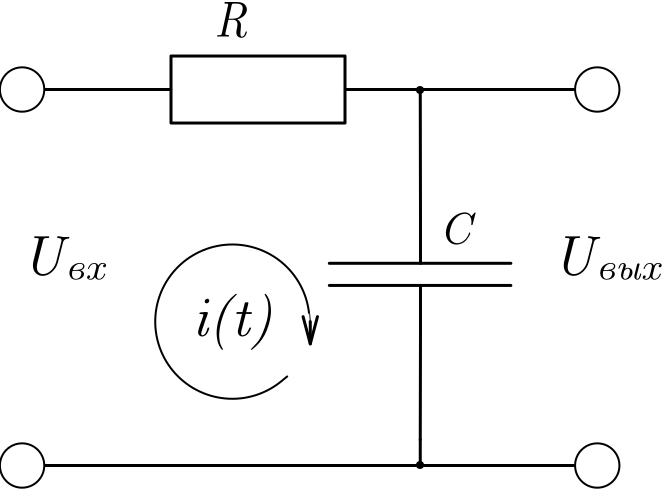
\includegraphics[width=0.8\linewidth]{graph/graph2}
		\caption{}
		\label{fig:1b}
	\end{subfigure}
	
	\caption{ }
	\label{fig:1}
\end{figure}

Поскольку дифференцирование и интегрирование -- линейные математические операции, то и на практике они осуществляются с помощью линейных четырехполюсников. Рассмотрим четырехполюсники, изображенные на \cref{fig:1}.

Подразумевая под входным сигналом электродвижущую силу, запишем уравнение второго закона Кирхгофа для этих схем:
\begin{align*}
	213
\end{align*}
\begin{equation} \label{eq:th:3}
	R i(t) + \frac{1}{C} \int\limits_{-\infty}^t i(t) \, dt = u_\text{вх}(t).
\end{equation}
Домножив это выржание на $C$ и считая, что произведение $RC$ равно постоянной времени цепи $\tau_0 = RC$, будем иметь:
\begin{equation} \label{eq:th:4}
	\tau_0 i(t) + \int\limits_{-\infty}^t i(t) \, dt = Cu_\text{вх}(t).
\end{equation}

Рассмотрим два крайних случая: очень малого и очень большого $\tau_0$. Если $\tau_0$ очень мало, то можно пренебречь первым слагаемым в \cref{eq:th:4}. Продифференцировав оставшиеся после отбрасывания этого слагаемого уравнение по $t$, получим:
\[i(t) \approx C\frac{du_\text{вх}(t)}{dt}.\]
Напряжение на резисторе $R$, пропорционально току, будет, в свою очередь, пропорционально производной от входного сигнала
\[u_R = Ri(t) \approx RC\frac{du_\text{вх}}{dt} = \tau_0 \frac{du_\text{вх}}{dt},\]
Таким образом, схема, приведенная на \cref{fig:1a}, у которой \(u_R = u_\text{вых}(t)\), может осуществлять приближенное дифференцирование входного сигнала.

При очень больших $\tau_0$ можно отбросить второе слагаемое в \cref{eq:th:4}. Тогда ток будет пропорционален входному сигналу
\[i(t) \approx \frac{C}{\tau_0} u_\text{вх}(t) = \frac{1}{R} u_\text{вх}(t),\]
а напряжение на конденсаторе
\[u_c = \frac{1}{C} \int\limits_{-\infty}^t i(t) \, dt \approx \frac{1}{RC} \int\limits_{-\infty}^t u_\text{вх}(t) \, dt = \frac{1}{\tau_0} \int\limits_{-\infty}^t u_\text{вх} (t) \, dt\]
пропорционально интегралу от входного сигнала. Такое преобразование может приближенно осуществлять четырехполюсник, приведенный на \cref{fig:1b}.

Уточним теперь приведенные выше понятия: малое и большое $\tau_0$.Проще всего это сделать на спектральном языке.

Известно, что практически все радиосигналы могут быть представлены в виде суперпозиции гармонических составляющих, в частности, для периодических сигналов -- в виде ряда Фурье:
\[u(t) = \frac{a_0}{2} + \sum\limits_{n=1}^\infty A_n \cos(n \Omega t - \theta_n).\]
Этот же ряд , если воспользоваться формулой Эйлера, может быть записан в комплексном виде
\[u(t) = \frac{1}{2} \sum\limits_{n=-\infty}^\infty \dot{A}_n e^{jn\Omega i},\]

где комплексная амплитуда $n$-ой гармоники определяется интегралом.
\[\dot{A}_n = \frac{2}{T} \int\limits_{-T/2}^{T/2} u(t) e^{-jn\Omega t} \, dt\]
Здесь $T$ -- период функции $u(t)$, связанный с угловой частотой соотношением $T = 2\pi / \Omega$.

Для непериодических сигналов аналогичные соотношения имеют вид:
\begin{align} \label{eq:th:5}
	u(t) = \frac{1}{2 \pi} \int_{-\infty}^{\infty} S(j\omega) e^{j\omega t} \, d\omega, &&
	S(j\omega) = \int_{-\infty}^\infty u(t) e^{-j\omega t} \, dt
\end{align}
Множитель $S(j\omega) = S(\omega) e^{j \varphi(\omega)}$ называют \textit{спектральной плотностью}.

\begin{figure}[t]
	\centering
	\begin{subfigure}[h]{0.49\linewidth}
		\centering
		\includegraphics[width=0.49\linewidth]{graph/graph2a}
		\includegraphics[width=0.49\linewidth]{graph/graph2b}
		\caption{}
		\label{fig:2a}
	\end{subfigure}
	\begin{subfigure}[h]{0.49\linewidth}
		\centering
		\includegraphics[width=0.49\linewidth]{graph/graph2c}
		\includegraphics[width=0.49\linewidth]{graph/graph2d}
		\caption{}
		\label{fig:2b}
	\end{subfigure}
	
	\caption{ }
	\label{fig:2}
\end{figure}

Связь между коэффициентами Фурье $\dot{A}_n$ и спектральной плотностью $S(j\omega)$ иллюстрируется рисунками \cref{fig:2a,fig:2b}, на первом из которых изображены амплитудная и фазовая спектральные диаграммы произвольной периодической последовательности импульсов, а на втором -- спектр одиночного импульса из этой последовательности. Форма огибающей на \cref{fig:2a} в некотором масштабе повторяет вид функции на \cref{fig:2b}.

Для четырехполюсников вводится также понятие коэффициента передачи --- комплексной функции вида
\[
K(j\omega) = \frac{\dot{U}_{\text{вых}}}{\dot{U}_{\text{вх}}} = K(\omega)e^{j\varphi(\omega)},
\]
где $\dot{U}_{\text{вх}}$ и $\dot{U}_{\text{вых}}$ --- комплексные амплитуды входного и выходного напряжения. (Напомним, что для сигнала вида $U(t) = U_0 e^{j(\omega t + \varphi)}$ комплексная амплитуда записывается в виде $\dot{U} = U_0 e^{j\varphi}$). Модуль $K(\omega)$ называют амплитудной характеристикой четырехполюсника, а аргумент $\varphi(\omega)$ --- фазовой характеристикой.

Каждая гармоника входного сигнала даст на выходе линейного четырехполюсника гармонический отклик той же частоты. Для его нахождения нужно эту гармонику умножить на коэффициент передачи четырехполюсника. Просуммировав отклики по всем гармоникам, можно определить выходной сигнал. В частности, для непериодических сигналов выражение для выходного сигнала запишется в интегральной форме:
\begin{equation} \label{eq:th:6}
	U_{\text{вых}}(t) = \frac{1}{2\pi}\int_{-\infty}^{\infty} S(j\omega)K(j\omega)e^{j\omega t}d\omega,
\end{equation}
где $S(j\omega)$ --- спектральная плотность входного сигнала.

Т.к. при дифференцированном напряжении $U_{\text{вых}} = \tau_0\frac{dU_{\text{вх}}}{dt}$, то используя \cref{eq:th:5,eq:th:6}, будем иметь:
\begin{multline*}
	U_{\text{вых}}(t) = \frac{1}{2\pi}\int_{-\infty}^{\infty} S(j\omega)K(j\omega)e^{j\omega t}d\omega =\\= \tau_0\frac{d}{dt}\left[\frac{1}{2\pi}\int_{-\infty}^{\infty} S(j\omega)e^{j\omega t}d\omega\right] = \tau_0\frac{1}{2\pi}\int_{-\infty}^{\infty} S(j\omega)j\omega e^{j\omega t}d\omega.
\end{multline*}

Из последнего равенства видно, что коэффициент передачи дифференцирующего четырехполюсника
\begin{equation} \label{eq:th:7}
	K(j\omega) = \tau_0 j\omega = \tau_0 \omega e^{j\pi/2}.
\end{equation}

Например, при дифференцировании гармонического напряжения типа $e^{j\omega t}$ выражение для выходного сигнала имеет вид:
\[
u_{\text{вых}}(t) = \tau_0 \frac{d}{dt} e^{j\omega t} = \tau_0 j\omega e^{j\omega t} = \tau_0 \omega e^{j\pi/2} e^{j\omega t}.
\]
Иными словами, для получения требуемого выходного сигнала каждая гармоника входного сигнала умножается на коэффициент $\tau_0 \omega$ и сдвигается по фазе на $\pi/2$.

Аналогичным образом для интегрирующей цепи можно получить

\begin{equation} \label{eq:th:8}
	K(j\omega) = \frac{1}{\tau_0 j\omega} = \frac{1}{\tau_0 \omega} e^{-\frac{j\pi}{2}}.
\end{equation}

Показанные на рис. \ref{fig:1a}, \ref{fig:1b} четырехполюсники имеют коэффициенты передачи
\begin{equation} \label{eq:th:9}
	K(j\omega) = \frac{R}{R + \frac{1}{j\omega C}} = RC  \frac{j\omega}{1 + RC j\omega} = \frac{\tau_0 j\omega}{1 + \tau_0 j\omega}.
\end{equation}
и
\begin{equation} \label{eq:th:10}
	K(j\omega) = \frac{\frac{1}{j\omega C}}{R + \frac{1}{j\omega C}} = \frac{1}{1 + j\omega CR} = \frac{1}{1 + \tau_0 j\omega}.
\end{equation}
соответственно.

Из сравнения выражений \eqref{eq:th:7} и \eqref{eq:th:9} следует, что для удовлетворительного дифференцирования необходимо выполнение условия:
\begin{equation} \label{eq:th:11}
	\tau_0 \omega \ll 1,
\end{equation}

а сравнивая выражения \eqref{eq:th:8} и \eqref{eq:th:10}, приходим к выводу, что удовлетворительное интегрирование возможно, если
\begin{equation} \label{eq:th:12}
	\tau_0 \omega \gg 1.
\end{equation}

Причем, эти условия должны выполняться для всех частот в существенной части спектра входного сигнала (говоря о существенной части спектра входного сигнала, имеется в виду, что теоретически спектр любого сигнала бесконечен).

Из этих неравенств вытекает также следующее принципиальное положение: чем точнее дифференцирование или интегрирование, тем меньше (по модулю) коэффициент передачи четырехполюсника, осуществляющего это преобразование. В пределе при идеальном преобразовании $K(\omega) \to 0$.

Собственно говоря, все предыдущие рассуждения о степени точности интегрирования или дифференцирования носили чисто качественный характер. Можно было бы, конечно, попытаться ввести какие-либо количественные критерии, но вряд ли стоит это делать. На практике все выглядит достаточно просто: есть конкретная задача о конкретном спектре, которую нужно продифференцировать или проинтегрировать с заданной степенью точности. Исходя из этого и выбирается параметр соответствующего четырехполюсника.

В заключение отметим, что рассмотренные выше модели дифференцирующих и интегрирующих цепей практически являются элементами более сложных электронных устройств. Как правило, для этих цепей применяются операционные усилители с обратной связью (в качестве элементов обратной связи и используются $R$, $C$---цепочки). В этом случае удается сочетать приемлемый коэффициент передачи с достаточно высоким качеством преобразования.